\PassOptionsToPackage{unicode=true}{hyperref} % options for packages loaded elsewhere
\PassOptionsToPackage{hyphens}{url}
%
\documentclass[12pt,english,]{article}
\usepackage{lmodern}
\usepackage{amssymb,amsmath}
\usepackage{ifxetex,ifluatex}
\usepackage{fixltx2e} % provides \textsubscript
\newcommand{\mtx}[1]{\begin{pmatrix}#1\end{pmatrix}} %Represents a matrix
\ifnum 0\ifxetex 1\fi\ifluatex 1\fi=0 % if pdftex
  \usepackage[T1]{fontenc}
  \usepackage[utf8]{inputenc}
  \usepackage{textcomp} % provides euro and other symbols
\else % if luatex or xelatex
  \usepackage{unicode-math}
  \defaultfontfeatures{Ligatures=TeX,Scale=MatchLowercase}
\fi
% use upquote if available, for straight quotes in verbatim environments
\IfFileExists{upquote.sty}{\usepackage{upquote}}{}
% use microtype if available
\IfFileExists{microtype.sty}{%
\usepackage[]{microtype}
\UseMicrotypeSet[protrusion]{basicmath} % disable protrusion for tt fonts
}{}
\usepackage{hyperref}
\hypersetup{
            pdfauthor={Thinh Truong},
            pdfborder={0 0 0},
            breaklinks=true}
\urlstyle{same}  % don't use monospace font for urls
\usepackage[margin=1in]{geometry}
\usepackage{graphicx,grffile}
\makeatletter
\def\maxwidth{\ifdim\Gin@nat@width>\linewidth\linewidth\else\Gin@nat@width\fi}
\def\maxheight{\ifdim\Gin@nat@height>\textheight\textheight\else\Gin@nat@height\fi}
\makeatother
% Scale images if necessary, so that they will not overflow the page
% margins by default, and it is still possible to overwrite the defaults
% using explicit options in \includegraphics[width, height, ...]{}
\setkeys{Gin}{width=\maxwidth,height=\maxheight,keepaspectratio}
\setlength{\emergencystretch}{3em}  % prevent overfull lines
\providecommand{\tightlist}{%
  \setlength{\itemsep}{0pt}\setlength{\parskip}{0pt}}
\setcounter{secnumdepth}{0}
% Redefines (sub)paragraphs to behave more like sections
\ifx\paragraph\undefined\else
\let\oldparagraph\paragraph
\renewcommand{\paragraph}[1]{\oldparagraph{#1}\mbox{}}
\fi
\ifx\subparagraph\undefined\else
\let\oldsubparagraph\subparagraph
\renewcommand{\subparagraph}[1]{\oldsubparagraph{#1}\mbox{}}
\fi
% set default figure placement to htbp
\makeatletter
\def\fps@figure{htbp}
\makeatother
\usepackage{float}
\usepackage[boxruled,vlined]{algorithm2e}
\usepackage{listings}
\usepackage{xcolor}
\usepackage {tikz}
\usepackage{indentfirst}
\usepackage{tabularx}
\usepackage{multirow}
\usepackage{pgfplots}
%\usepackage[bottom]{footmisc}
\colorlet{mygray}{black!30}
\colorlet{mygreen}{green!60!black}
\colorlet{mymauve}{red!90}
\lstset{
  tabsize=2,
  backgroundcolor=\color{gray!10},  
  basicstyle=\ttfamily,
  columns=fullflexible,
  breakatwhitespace=false,      
  breaklines=true,                
  captionpos=b,                    
  commentstyle=\color{mygreen}, 
  extendedchars=true,              
  frame=single,                   
  keepspaces=true,             
  keywordstyle=\bfseries\color{blue},      
  language=c++,                 
  numbers=left,                
  numbersep=5pt,
  breaklines=true,
  numberstyle=\tiny, 
  rulecolor=\color{mygray},        
  showspaces=false,               
  showtabs=true,                                  
  stringstyle=\color{mymauve},                          
  title=\lstname                
}
\definecolor{light-gray}{gray}{0.9}
\newcommand{\code}[1]{\colorbox{light-gray}{\texttt{#1}}}
\newcommand{\pnt}[1]{{\scriptstyle#1}}
\let\origfigure\figure
\let\endorigfigure\endfigure
\renewenvironment{figure}[1][2] {
    \expandafter\origfigure\expandafter[H]
} {
    \endorigfigure
}
\usepackage{etoolbox}
\makeatletter
\providecommand{\subtitle}[1]{% add subtitle to \maketitle
  \apptocmd{\@title}{\par {\large #1 \par}}{}{}
}
\makeatother
\ifnum 0\ifxetex 1\fi\ifluatex 1\fi=0 % if pdftex
  \usepackage[shorthands=off,main=english]{babel}
\else
  % load polyglossia as late as possible as it *could* call bidi if RTL lang (e.g. Hebrew or Arabic)
  \usepackage{polyglossia}
  \setmainlanguage[]{english}
\fi
\title{\textbf{Project Report}\\
\Large{An Experimentation Of:}}
\providecommand{\subtitle}[1]{}
\subtitle{Cloning a node in XOR model}
\author{Thinh Truong \\ Supervised by Dr. Yuly Billig}
\date{11 August 2021}

% Input layer neurons'number
\newcommand{\inputnum}{2} 
 
% Hidden layer neurons'number
\newcommand{\hiddennum}{2}  
 
% Output layer neurons'number
\newcommand{\outputnum}{1} 

\begin{document}
\maketitle

\hypertarget{section1}{%
\section{\texorpdfstring{1
\enspace Introduction}{1 Introduction}}\label{section1}}

The XOR problem is a classic problem in machine learning. However, a model with a hidden layer of two nodes may not product correct predictions and it depends a lot on the initial weights and biases. Therefore, in order to tackle this problem, one must increase the number of nodes in the hidden layer. In this report, I will explain the idea behind cloning a node, and point out the problems that I encountered with it.

In the XOR problem, given a model with two nodes in input layer, two nodes in hidden layer and one node in output layer, we can think of the following model. 

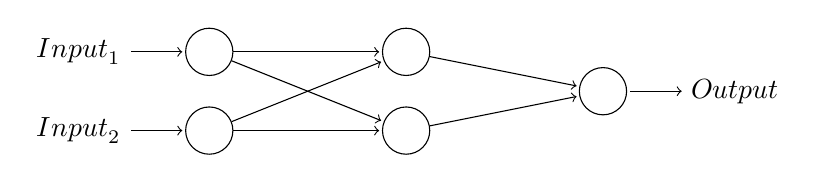
\begin{tikzpicture}
 
% Input Layer
\foreach \i in {1,...,\inputnum}
{
    \node[circle, 
        minimum size = 6mm,
         fill=white!100, draw=black] (Input-\i) at (0,-\i) {};
}
 
% Hidden Layer
\foreach \i in {1,...,\hiddennum}
{
    \node[circle, 
        minimum size = 6mm,
         fill=white!100, draw=black,
        yshift=(\hiddennum-\inputnum)*5 mm
    ] (Hidden-\i) at (2.5,-\i) {};
}
 
% Output Layer
\foreach \i in {1,...,\outputnum}
{
    \node[circle, 
        minimum size = 6mm,
         fill=white!100, draw=black,
        yshift=(\outputnum-\inputnum)*5 mm
    ] (Output-\i) at (5,-\i) {};
}
 
% Connect neurons In-Hidden
\foreach \i in {1,...,\inputnum}
{
    \foreach \j in {1,...,\hiddennum}
    {
        \draw[->, shorten >=1pt] (Input-\i) -- (Hidden-\j);   
    }
}
 
% Connect neurons Hidden-Out
\foreach \i in {1,...,\hiddennum}
{
    \foreach \j in {1,...,\outputnum}
    {
        \draw[->, shorten >=1pt] (Hidden-\i) -- (Output-\j);
    }
}
 
% Inputs
\foreach \i in {1,...,\inputnum}
{            
    \draw[<-, shorten <=1pt] (Input-\i) -- ++(-1,0)
        node[left]{$Input_{\i}$};
}
 
% Outputs
\foreach \i in {1,...,\outputnum}
{            
    \draw[->, shorten <=1pt] (Output-\i) -- ++(1,0)
        node[right]{$Output$};
}
 
\end{tikzpicture}

Throughout the paper, let:

\vspace{-2truemm}

\begin{quote}
\begin{itemize}
\item The input layer be layer 1, the hidden layer be layer 2, and the output layer be layer 3.
\item The learning rate $\epsilon$ be 1 to speed up training.
\item $w_{jk}^{l}$ be the weight from the $k^{th}$ node in the $(l-1)^{th}$ layer to the $j^{th}$ node in the $l^{th}$ layer.
\item $b_{j}^l$ be the bias of the $j^{th}$ node in the $l^{th}$ layer.
\item $z_{j}^l$ be the weighted input of the $j^{th}$ node in the $l^{th}$ layer and\\ $z_{j}^{l} =\sum_{k}w_{jk}^{l}a_{k}^{l-1} + b_{j}^l$
\item $a_{j}^l$ be the activation of the $j^{th}$ node in the $l^{th}$ layer and\\ $a_{j}^{l} =\sigma(\sum_{k}w_{jk}^{l}a_{k}^{l-1} + b_{j}^l)= \sigma(z_{j}^{l})$.
\end{itemize}
\end{quote}

\vspace{-2truemm}

\newpage

Using the above notations, we therefore get the following matrices for our XOR model.

\begin{align*}
\text{Weight matrix 1} &&\text{Bias matrix 1} \\
\mtx{w_{11}^2 & w_{12}^2\\  w_{21}^2 & w_{22}^2} &&\mtx{b_{1}^2 \\ b_{2}^2 }\\
\text{Weight matrix 2} &&\text{Bias matrix 2}\\
\mtx{w_{11}^3 & w_{12}^3} &&\mtx{b_{1}^3}\\
\end{align*}

\hypertarget{section2}{%
\section{\texorpdfstring{2 \enspace Cloning a node}{2 Cloning a node}}\label{section2}}

\hypertarget{section2.1}{%
\subsection{\texorpdfstring{2.1 \enspace The case where our model would not produce correct \\ predictions}{2.1 The case where our model would not produce correct predictions}}\label{section2.1}}

One case where training our two-node hidden layer model would not work is when the weights and biases are initialized as below:

\begin{align*}
\text{Weight matrix 1} &&\text{Bias matrix 1} \\
\mtx{4 & -6\\  -4 & -5} &&\mtx{-3 \\ 0.5}\\
\text{Weight matrix 2} &&\text{Bias matrix 2}\\
\mtx{4 & -4} &&\mtx{0}\\
\end{align*}

The following image is the prediction of our initial model for all four cases.

\begin{figure}

{\centering 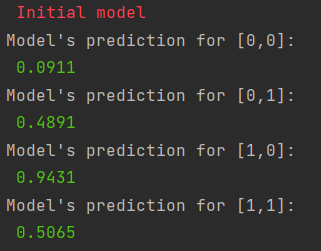
\includegraphics[width=0.7\linewidth]{images/initial_pred} 

}

\caption{\label{fig1:figs}The predictions of the initial model.}\label{fig:unnamed-chunk-1}
\end{figure}

\hrule

~

~

This model starts with good predictions for [0,0] and [1,0] cases and bad predictions for the other two cases (see Figure \ref{fig1:figs}). However, as we train the model, we will never get the predictions we expected . I choose $50000$ epochs because it is a large enough number to show that the cost function will never converge to zero.

\begin{figure}

{\centering 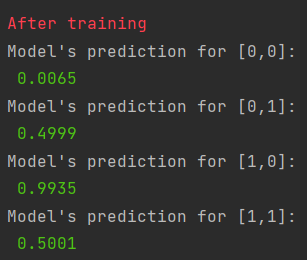
\includegraphics[width=0.7\linewidth]{images/50k_pred} 

}

\caption{\label{fig2:figs}The predictions of the model after $50 000$ epochs.}\label{fig:unnamed-chunk-2}
\end{figure}

~

\begin{figure}

{\centering 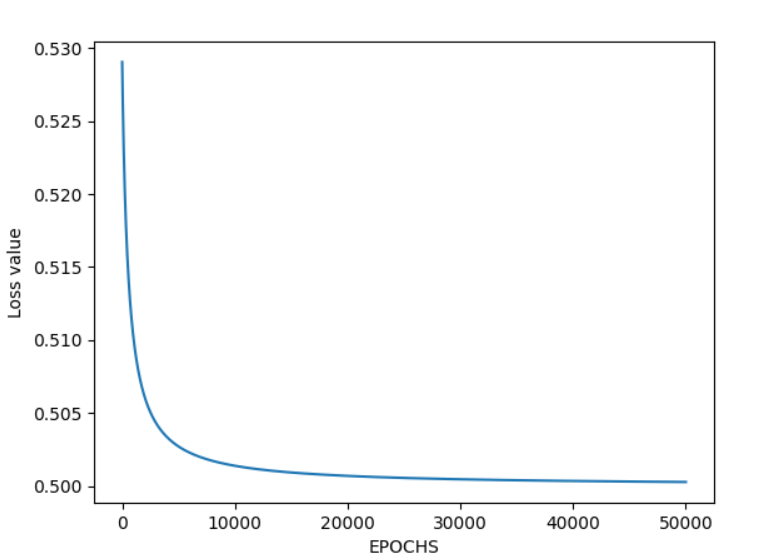
\includegraphics[width=0.7\linewidth]{images/50k_graph} 

}

\caption{\label{fig3:figs}The graph of cost function after $50 000$ epochs.}\label{fig:unnamed-chunk-3}
\end{figure}

\hrule

~
 
\hypertarget{section2.2}{%
\subsection{\texorpdfstring{2.2 \enspace The theory of cloning a node}{2.2 The theory of cloning a node}}\label{section2.2}}

In order to overcome local minimum in the above model, we can add a node in the hidden layer so that there is a new dimension in our cost function.  Cloning a node means we copy a node from the hidden layer, and create an exact same node with the same input weights and bias, but decrease the output weights of both nodes by half. The reason we have to halve the output weights is because we would want to maintain all the features from the previous model, and so, to keep  $a_{1}^{3}$ the same after adding a new node with the same activation as the original node, the output weights must be reduced by half. 

In this case, let us clone the second node in the hidden layer from the initial model, where we skip training the model for $50000$ epochs, and place the new node in the third position. This results in a new model with three nodes in the hidden layer and the following weight and bias matrices

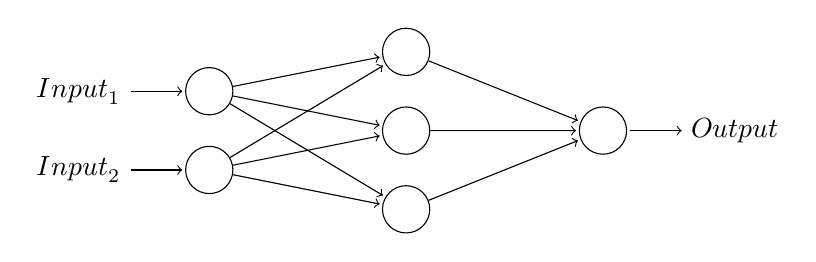
\begin{tikzpicture}
 
% Input Layer
\foreach \i in {1,...,2}
{
    \node[circle, 
        minimum size = 6mm, fill=white!100,draw=black] 
	(Input-\i) at (0,-\i) {};
}
 
% Hidden Layer
\foreach \i in {1,...,3}
{
    \node[circle, 
        minimum size = 6mm,
         fill=white!100, draw=black,
        yshift=(3-2)*5 mm
    ] (Hidden-\i) at (2.5,-\i) {};
}
 
% Output Layer
\foreach \i in {1}
{
    \node[circle, 
        minimum size = 6mm,
         fill=white!100, draw=black,
        yshift=(1-2)*5 mm
    ] (Output-\i) at (5,-\i) {};
}
 
% Connect neurons In-Hidden
\foreach \i in {1,...,2}
{
    \foreach \j in {1,...,3}
    {
        \draw[->, shorten >=1pt] (Input-\i) -- (Hidden-\j);   
    }
}
 
% Connect neurons Hidden-Out
\foreach \i in {1,...,3}
{
    \foreach \j in {1}
    {
        \draw[->, shorten >=1pt] (Hidden-\i) -- (Output-\j);
    }
}
 
% Inputs
\foreach \i in {1,...,2}
{            
    \draw[<-, shorten <=1pt] (Input-\i) -- ++(-1,0)
        node[left]{$Input_{\i}$};
}
 
% Outputs
\foreach \i in {1}
{            
    \draw[->, shorten <=1pt] (Output-\i) -- ++(1,0)
        node[right]{$Output$};
}
 
\end{tikzpicture}

\begin{align*}
\text{Weight matrix 1} &&\text{Bias matrix 1}\\
\mtx{4 & -6\\  -4 & -5 \\ -4 & -5} &&\mtx{-3 \\ 0.5 \\ 0.5 }\\
\text{Weight matrix 2} &&\text{Bias matrix 2}\\
\mtx{4 & -2 &  -2} &&\mtx{0}\\
\end{align*}

Therefore, as expected, we would get the same predictions as the as before.

\begin{figure}

{\centering 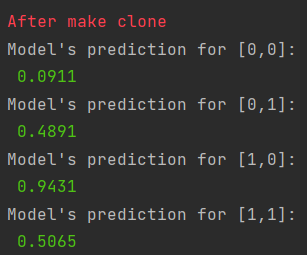
\includegraphics[width=0.7\linewidth]{images/initial_clone_pred} 

}

\caption{\label{fig4:figs}The prediction of the model after cloning a node.}\label{fig:unnamed-chunk-4}
\end{figure}

\hrule

~

~

However, if we keep training our model with the normal backpropagation method, the two copies of the cloned node will always be updated in the same way and that would make our new node pointless. Therefore, initially, we would have to distinguish the two copies. In this report, let consider $\dfrac{\delta C}{\delta a_{j}^{l}}$ as the auxilary partial derivative of the $j^{th}$ node in the $l^{th}$ layer . Thus, I alternate updating the partial derivatives of the cost function with respect to weights and biases of each node based on their auxilary partial derivative. 

\begin{figure}[ht]
  \centering
  \begin{minipage}{.9\linewidth}
    {\LinesNotNumbered
    \SetAlgoRefName{}
    \begin{algorithm}[H]
    \SetKwInOut{Input}{Input}
    \Input{Let $e$ be the position of the original node, $f$ be the position of the new node in the hidden layer $l$.}
    \SetKwInOut{Output}{Output}
    \Output{Update the original node when its auxilary partial derivative is positive and update the new node when its auxilary partial derivative is negative.}
    \SetAlgoLined
    \BlankLine
    \centering
    \begin{minipage}{.75\linewidth}
        \uIf{$\dfrac{\delta C}{\delta a_{e}^{l}} < 0$} {
            $\dfrac{\delta C}{\delta b_{e}^{l}} = 0$\\
	    \For{k be each node number in the input layer} {
		$\dfrac{\delta C}{\delta w_{ek}^{l}} = 0$
	    }
	    \For{j be each node number in the output layer} {
		$\dfrac{\delta C}{\delta w_{je}^{l+1}} = 0$
	    }
        }
	\uIf{$\dfrac{\delta C}{\delta a_{f}^{l}} > 0$} {
            $\dfrac{\delta C}{\delta b_{f}^{l}} = 0$\\
	    \For{k be the node number in the input layer} {
		$\dfrac{\delta C}{\delta w_{fk}^{l}} = 0$
	    }
	    \For{j be the node number in the output layer} {
		$\dfrac{\delta C}{\delta w_{jf}^{l+1}} = 0$
	    }
        }	
    \end{minipage}
    \caption{\textsc{Alternating node update method}}
    \end{algorithm}}
  \end{minipage}
\end{figure}

After training the model with this method a certain number of epochs, the two copies of the cloned nodes will be two distinguishable nodes and we then can proceed to train the model normally. With the new node in the hidden layer, we essentially add a new dimension for the cost function to overcome the local minimum, and expect the new model will perform well with the predictions.

\newpage

\hypertarget{section3}{%
\section{\texorpdfstring{3 \enspace Current obstacles with cloning a node}{3 Current obstacles with cloning a node}}\label{section3}}

With the alternating node update method, initially, the cost value goes down, as expected. We would expect the graph of the cost function to continue decreasing while the two nodes are differentiated. However, after around 300 epochs, the curve starts to increase, which reaches the peak at around $2700$ epochs and then plunges and stays stabilized after that. 


\begin{figure}

{\centering 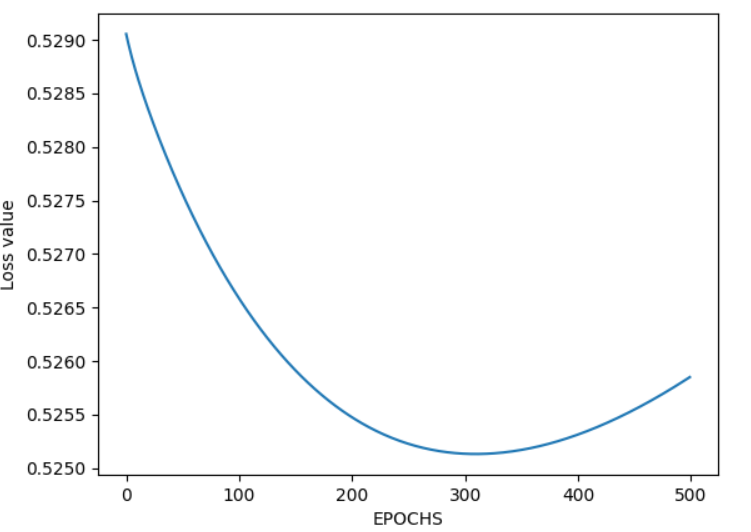
\includegraphics[width=0.7\linewidth]{images/500_graph} 

}
\caption{\label{fig5:figs}The graph of cost function after $500$ epochs trained with alternating node update method.}\label{fig:unnamed-chunk-4}
\end{figure}

\begin{figure}

{\centering 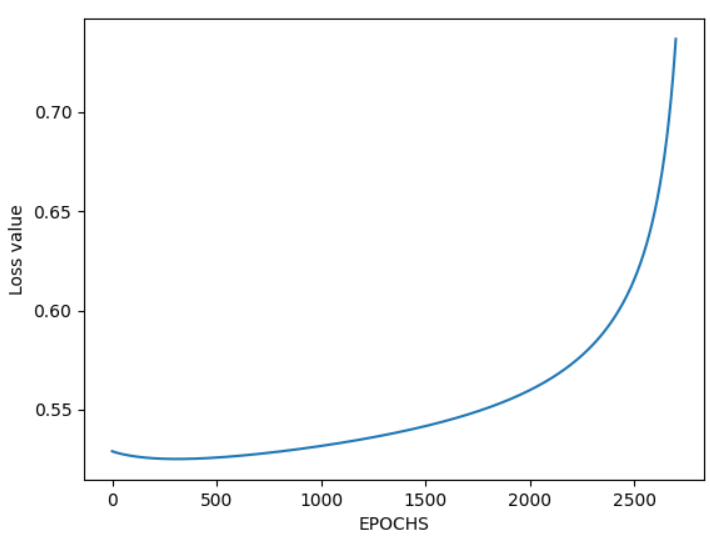
\includegraphics[width=0.7\linewidth]{images/2k7_graph} 

}
\caption{\label{fig5:figs}The graph of cost function after $2700$ epochs trained with alternating node update method.}\label{fig:unnamed-chunk-5}
\end{figure}

\begin{figure}

{\centering 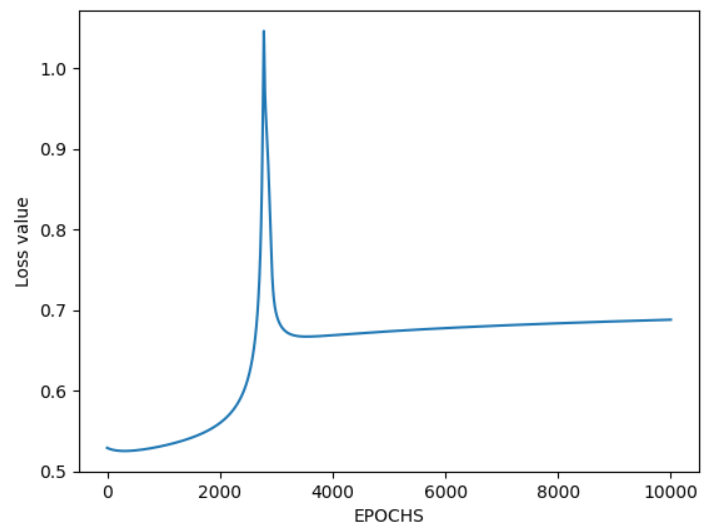
\includegraphics[width=0.7\linewidth]{images/10k_graph} 

}

\caption{\label{fig6:figs}The graph of cost function after $10 000$ epochs trained with alternating node update method.}\label{fig:unnamed-chunk-6}
\end{figure}

\hrule

~

~

\newpage

The resulting graphs produce a surprising behavior of the cost function. As of now, I cannot mathematically reason why it does behave this way. However, there are a few things that I have observed during the training.

Let consider the $\dfrac{\delta C}{\delta w_{jk}^{l}}$ matrices and $\dfrac{\delta C}{\delta b_{j}^{l}}$ matrices of the initial model, model after $200$ epochs and after $400$ epochs.

~

\code{Initial model}

Alternating node update method
\begin{align*}
\text{$\dfrac{\delta C}{\delta w_{jk}^{l}}$ matrix 1} &&\text{$\dfrac{\delta C}{\delta b_{j}^{l}}$ matrix 1}\\
\mtx{0.001922699 & 0.006607202\\  0.00034808 & 0.005548522 \\ -0.000102995 & -0.000102995} &&\mtx{0.00452357 \\ 0.005896602 \\ -0.007195426 }\\
\text{$\dfrac{\delta C}{\delta w_{jk}^{l}}$ matrix 2} &&\text{$\dfrac{\delta C}{\delta b_{j}^{l}}$ matrix 2}\\
\mtx{-0.002092904 & -0.002984376 &  0.009444445} &&\mtx{0.006864792}\\
\end{align*}

Normal trainning method
\begin{align*}
\text{$\dfrac{\delta C}{\delta w_{jk}^{l}}$ matrix 1} &&\text{$\dfrac{\delta C}{\delta b_{j}^{l}}$ matrix 1}\\
\mtx{0.001922699 & 0.006607202\\  0.000245085 & 0.005445527 \\ 0.000245085 & 0.005445527} &&\mtx{0.00452357 \\ -0.001298824 \\ -0.001298824 }\\
\text{$\dfrac{\delta C}{\delta w_{jk}^{l}}$ matrix 2} &&\text{$\dfrac{\delta C}{\delta b_{j}^{l}}$ matrix 2}\\
\mtx{-0.002092904 & 0.006460069 &  0.006460069} &&\mtx{0.006864792}\\
\end{align*}

\code{After 200 epochs}

Alternating node update method
\begin{align*}
\text{$\dfrac{\delta C}{\delta w_{jk}^{l}}$ matrix 1} &&\text{$\dfrac{\delta C}{\delta b_{j}^{l}}$ matrix 1}\\
\mtx{-0.000589661 & 0.004670982\\  0.000264909 & 0.003371733 \\ -0.000168785 & -0.000168785} &&\mtx{0.000988999 \\ 0.003636642 \\ -0.005198084 }\\
\text{$\dfrac{\delta C}{\delta w_{jk}^{l}}$ matrix 2} &&\text{$\dfrac{\delta C}{\delta b_{j}^{l}}$ matrix 2}\\
\mtx{-0.002882543 & -0.001950929 &  0.006852048} &&\mtx{-0.000386748}\\
\end{align*}

Normal trainning method
\begin{align*}
\text{$\dfrac{\delta C}{\delta w_{jk}^{l}}$ matrix 1} &&\text{$\dfrac{\delta C}{\delta b_{j}^{l}}$ matrix 1}\\
\mtx{-0.000589661 & 0.004670982\\  0.000204223 & 0.003311048 \\ 0.000401603 & 0.008857716} &&\mtx{0.000988999 \\ -0.000955161 \\ 0.004398805 }\\
\text{$\dfrac{\delta C}{\delta w_{jk}^{l}}$ matrix 2} &&\text{$\dfrac{\delta C}{\delta b_{j}^{l}}$ matrix 2}\\
\mtx{-0.002882543 & 0.003645883 &  0.002783048} &&\mtx{-0.000386748}\\
\end{align*}

\code{After 400 epochs}

Alternating node update method
\begin{align*}
\text{$\dfrac{\delta C}{\delta w_{jk}^{l}}$ matrix 1} &&\text{$\dfrac{\delta C}{\delta b_{j}^{l}}$ matrix 1}\\
\mtx{-0.000705775 & 0.003942532\\  0.000184971 & 0.002402513 \\ -0.000243775 & -0.000243775} &&\mtx{0.000396406 \\ 0.002587484 \\ -0.003846889 }\\
\text{$\dfrac{\delta C}{\delta w_{jk}^{l}}$ matrix 2} &&\text{$\dfrac{\delta C}{\delta b_{j}^{l}}$ matrix 2}\\
\mtx{-0.002585391 & -0.001450028 &  0.005161626} &&\mtx{-0.00027088}\\
\end{align*}

Normal trainning method
\begin{align*}
\text{$\dfrac{\delta C}{\delta w_{jk}^{l}}$ matrix 1} &&\text{$\dfrac{\delta C}{\delta b_{j}^{l}}$ matrix 1}\\
\mtx{-0.000705775 & 0.003942532\\  0.000141997 & 0.002359538 \\ 0.000434988 & 0.012453106} &&\mtx{0.000396406 \\ -0.000536601 \\ 0.009528755 }\\
\text{$\dfrac{\delta C}{\delta w_{jk}^{l}}$ matrix 2} &&\text{$\dfrac{\delta C}{\delta b_{j}^{l}}$ matrix 2}\\
\mtx{-0.002585391 & 0.002216078 &  9.65872\cdot10^{-5}} &&\mtx{-0.00027088}\\
\end{align*}

As we see, even from the initial model, the gradients of the third node in the $\dfrac{\delta C}{\delta w_{jk}^{l}}$ matrix 1 are positive numbers if we train the model normally. However, due to the way how we update the new node (third node) when we train the model with the alternating node update method,  the gradients of the third node in the $\dfrac{\delta C}{\delta w_{jk}^{l}}$ matrix 1 are negative numbers, which means we would then update the weights of the third node in the direction that would increase the value of the cost function the most. As the number of epochs increases and we keep updating the weights of the third node in the opposite direction of the normal training method, the gradients of the third node in the $\dfrac{\delta C}{\delta w_{jk}^{l}}$ matrix 1 in later epochs become large positive numbers. Therefore, it makes some predictions worse, especially the [1,1] case where the output depends a lot on the weights of the third node, and so, the graph of the cost functions would start to increase.

\hypertarget{section4}{%
\section{\texorpdfstring{4 \enspace Concluding
remarks}{4 Concluding remarks}}\label{section4}}

I have briefly described the theory of cloning a node, and the implementation of it. Although it works as expected initially, the graph of the cost function eventually blows up before we can reach the target predictions with the normal training method. Therefore, there is still a question whether it is efficient to clone a node to keep the features from the previous training that may be modified during the alternating node update method before the target predictions are reached?

























\end{document}
